
\chapter{Conclusion}\label{chap:conclusion}

Bayesian methods provide a powerful framework for quantifying uncertainty in ozone
combustion applications. Bayesian calibration, given a set of experimental data of flame speed to compare
against, both improves calibration of the chemical kinetic parameter as well as providing
updated distributions for the parameters. Those distributions can then be
propagated forward into simulations of laminar flame speed to determine the uncertainty in
their predictions. The application of this approach to existing experimental data of flame speed for ozone combustion model was done here.


We made a detailed discussion on the mathematical models used for combustion for both multi dimensional and one dimensional reacting-flow . In this work, we used the mathematical model developed for 1D free flame~\cite{Kuo}. For different concentrations of ozone from the experimental data by Steng~\cite{Streng}, Cantera~\cite{Cantera} was used to solve for forward model and calculate the flamespeed. We have justified our use of surrogate model to reduce  sampling load. The sample and surrogates have good convergence. The use linear surrogate models to calculate the flame speed values at different points in the domain can be improved by taking higher order approximations. As a sanity check, We have ensured that the samples which we are drawing actually fit the data of flamespeed from the experiments of Streng\cite{Streng}. Finally we have studied the mean and autocorrelation plots for the distribution. We have seen that more number of surrogate points are required to obtain better probability distribution distribution for parameters. Also we need more MCMC samples to get better statistical results. As we increase the domain size for the parameters, we encounter numerical difficulties for our forward run. The newton iterations do not converge. Investigations need to be done for $17$, $20 \% $and $ 28 \% $ percent ozone case. There is numerical difficulties for calculating the flame speed for these cases. We need to investigate these difficulties. 

In future, We would like to add more statistical model to our work i.e do the UQ analysis with three or four unknown parameters of the ozone mechanism. In this way, we can develop a good mathematical model for combustion. It would be interesting to do similar work for diffusion flames where fuel and oxygen are not mixed initially.. We would like to generalize this approach to multidimensional combustion where we could include Bunsen burner flame and do uncertainty quantification for 2D or even 3D laminar flame speeds.  


We end our work with  framework for doing Bayesian inference for 2D premixed laminar flames. We have been working towards development of finite element models for 2D premixed Bunsen burner flame. The future work will involve the doing the uncertainty quantification for these 2D flames. There are various numerical stability problems which we need to address in this case. Moving ahead good statistical finite element model can serve as good foundation for doing Bayesian inference. We can also include parameters like viscosity and  thermal conductivity for uncertainty involved in transport model. The figure~\ref{amr_flame} shows the adaptive mesh refinement method for the 2D flame. Here the initial concentration of ozone is 20 $\%$.  The plot shows the temperature variation in the 2D domain. We have used open source C++ library GRINS~\cite{GRINSPaper}.

 \begin{figure}[h]
   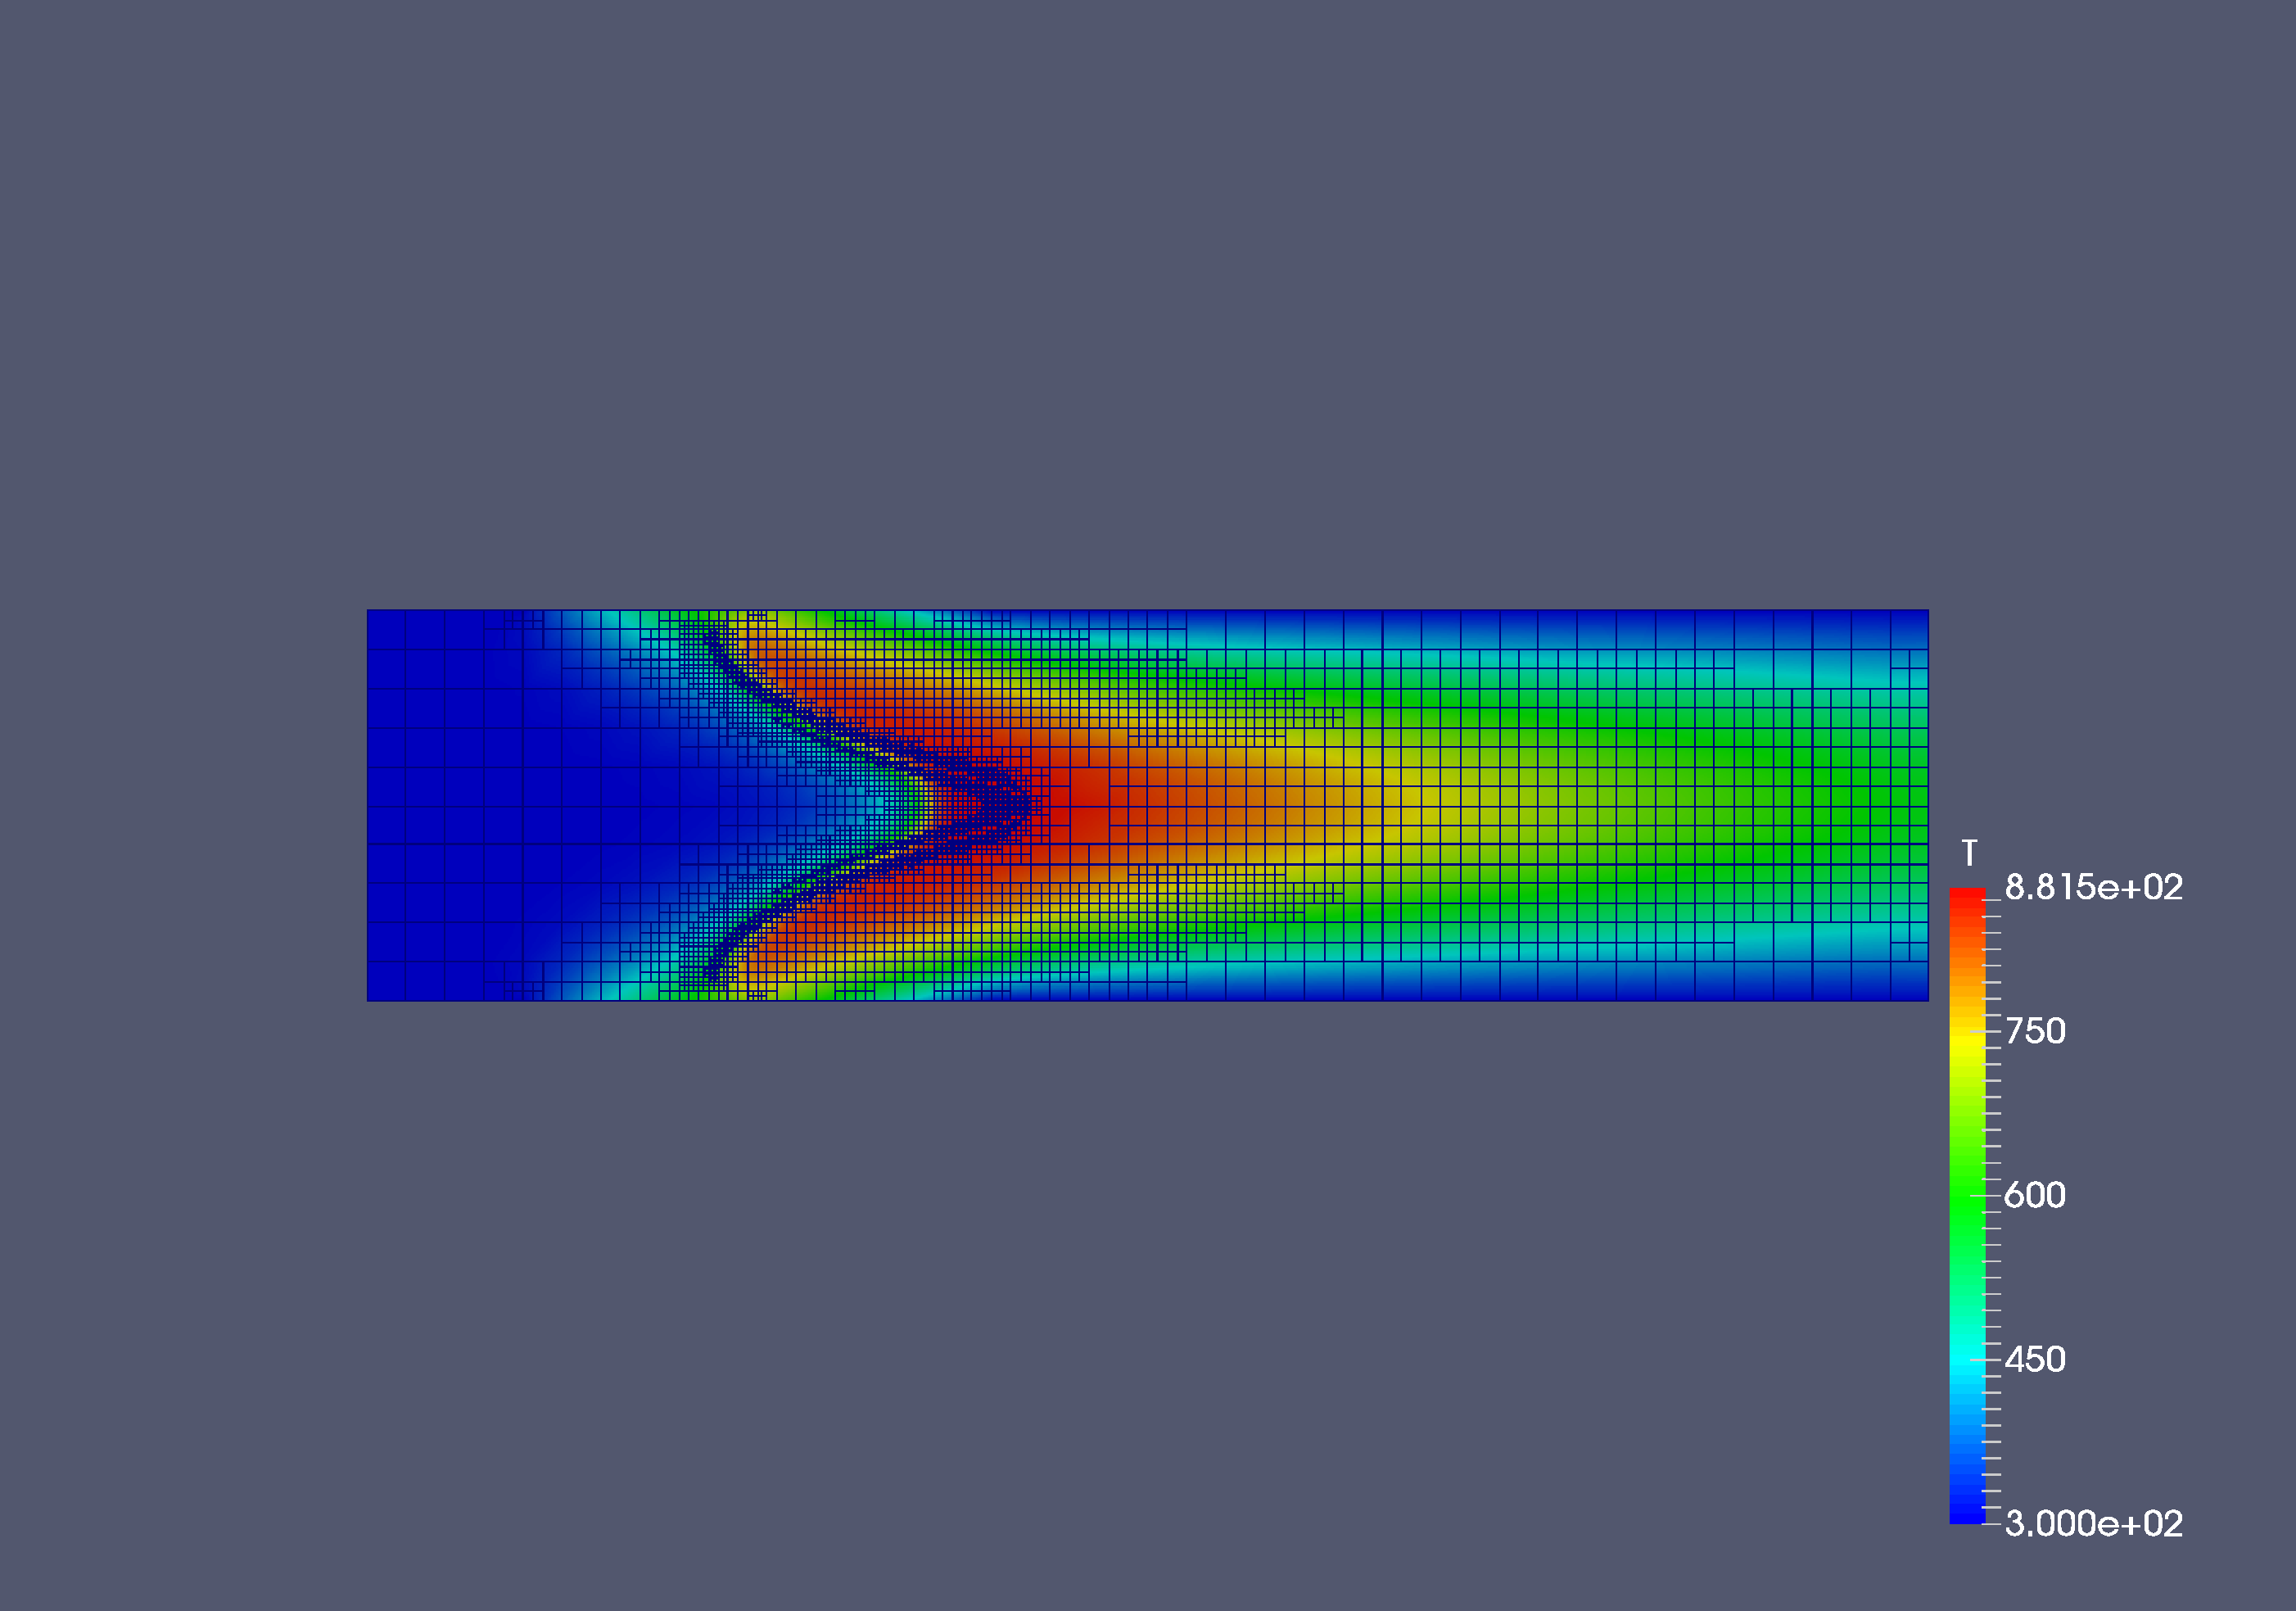
\includegraphics[scale=0.35]{figs/flame_amr.pdf}
    \caption{2D flame}
    \label{amr_flame}
 \end{figure}

